\section{The Invariant Framework}

Given the many challenges of reproducing HEP applications, we now describe an invariant framework, which if present within large collaborations, can enable application developers to share their 
application with other researchers, and for other researchers to reproduce the shared application. 
To satisfy invariance, the framework must include mechanisms for:

\begin{itemize}

\item {\bf Capturing Dependencies and Configurations:} Capturing tools must record dependencies that are used by the program, including hardware, OS, kernels, static and dynamic dependencies, local and networked dependencies, source codes and data files. Stateful interactions with commercial software, such as proprietary databases and which cannot be captured due to licensing agreements must be persisted so that they can replayed later without the presence of the commercial software.  In effect, a captured application should behave exactly the same way as the application developer intended it to be. 
% In audit phase, PTU captures the execution of the application into a package. The resulting package contains the source code, its dependencies (system files, and files on network such as from CernVM-FS) and the data consumed and written by the application.

\item{\bf Preservation of Captured Entities:} By preservation we imply appropriate mechanisms for (a) documentation of the application development, and (b) automation of any task that becomes inevitably 
necessary for repeating the application in exactly the same way as the developer executed it. 
 
Documentation and specification during application development can be an onerous one. The preservation framework must make programming tools available that 
focus less on documentation, but script, integrate and execute the dependencies so that they are resolved as part of documentation. 
Automation can extend to various tasks that are necessary for ensuring repeatability such as building software, provisioning of hardware, 
validation of software against security fixes, new features, and even monitoring the reproducibility state of a preserved application, i.e., its source code, dependencies, environment, and platform.
Automated builds and provisioning and continuous integration service can significantly lower the barrier to run the application in a new environment. 

In spite of the preservation mechanisms, the application software may not run as intended. For a reproducer's understanding, it may also be useful to include 
a \emph{logical preservation unit} (PLU) that consists of a minimal execution of the software using a small, test data sample, and with specified outputs.
The provenance of this PLU must be captured so that the reproducer can make comparison with future reproduction-validation runs. 

\item {\bf Distribution of Preserved Packages:} A captured and preserved application must be persistently stored and distributed through a repository. We imagine these repositories to be themselves preserved, and linked with a digital library. Metadata and flexible annotation should be part of this repository for curation over time. 

\end{itemize}


%\section{Evolving the Artifact}
%
%\begin{figure*}[t]
%\centering
%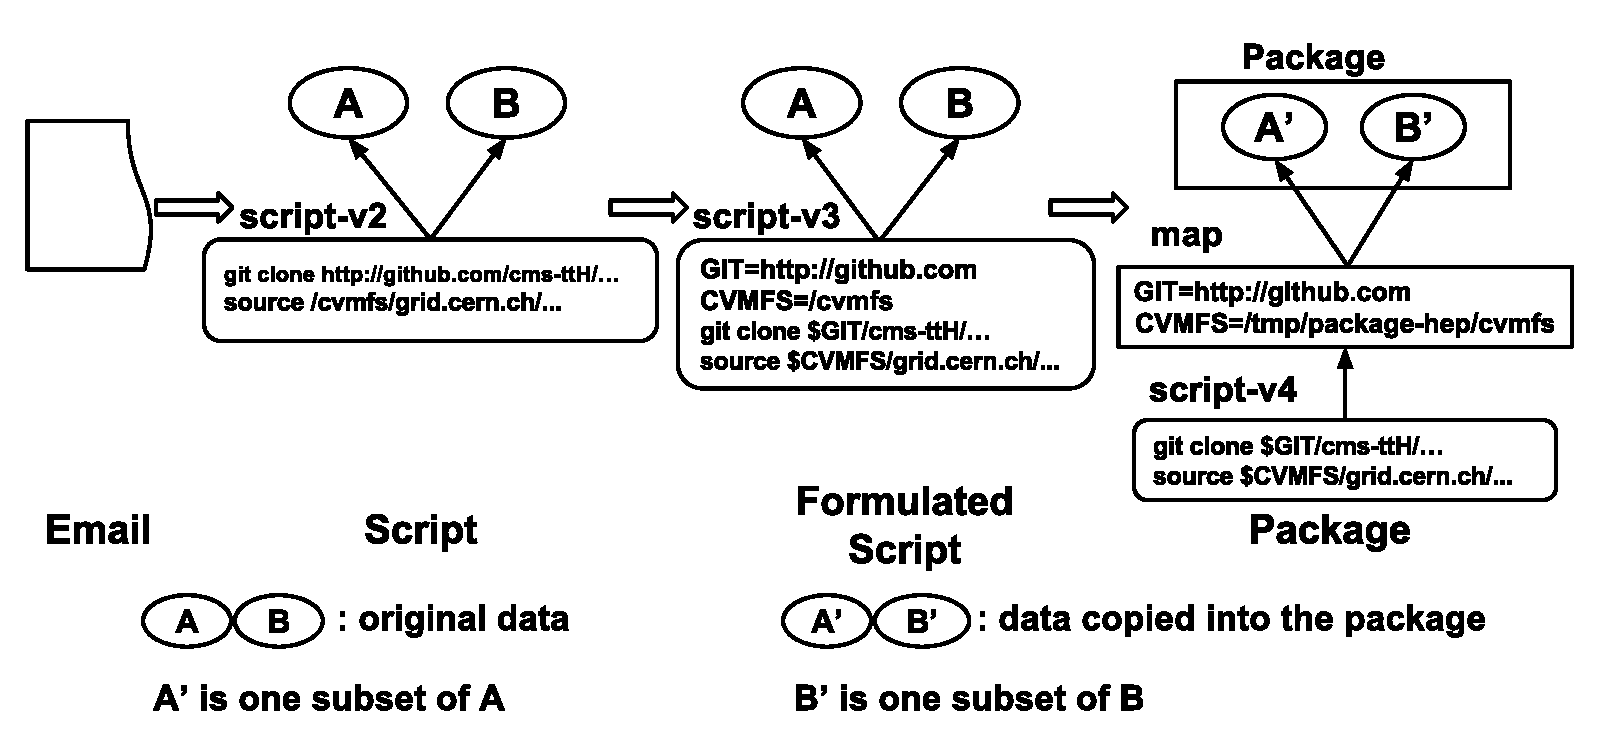
\includegraphics[width=.8\textwidth]{version-evolution.eps}
%\caption{Version Evolution}
%\label{fig:version-evolution}
%\end{figure*}
%
%It is clear that the artifact, as provided, is not in a suitable form
%for preservation.  While it might be technically possible to automatically
%capture the entire virtual machine and all of the connected filesystems,
%it would require 166.8TB of storage, which would be prohibitively expensive
%for capturing this one application alone.  Further, if multiple
%similar applications are preserved, we would miss the opportunity to identify
%common dependencies and store them once for multiple artifacts.
%A more structured approach to dependency management is needed.
%
%Figure~\ref{fig:version-evolution} shows how we have evolved this artifact
%through several stages which make it more suitable for preservation.
%In each step of evolution, we make the dependencies of the artifact
%more explicit and available for analysis and automated processing.
%As noted in the previous section, the original author provided us with
%prose instructions by email which we translated into an
%executable script.  The executable script has embedded in it
%a number of external identifiers such as URLs pointing to repositories
%and paths to networked filesystems.  As a general programming practice,
%embedding such constants into the middle of a program is unwise, and so
%we extract all of those identifiers and place them \emph{outside} the
%script in a \emph{dependency map} or just \emph{map} for short.
%The dependency map lists all of the external dependencies of the application, indicating
%the type, how they are accessed, and where they are currently located.
%The resulting script then simply refers to abstract file locations such
%as \verb$GIT$ and \verb$CVMFS$, while the map file indicates where they
%are currently located. If properly constructed, the script should not refer to any external
%resource unless it is indicated in the dependency map.  We call this idealized
%artifact an \emph{abstract script}.
%
%By extracting the dependencies into the dependency map,
%we introduce great freedom for the curator to move, transform, and otherwise
%manipulate the dependencies of the artifact without damaging the artifact itself.
%A Figure~\ref{fig:version-evolution} shows, it is straightforward for an
%automated tool to examine
%all of the dependencies in the map, download those that are missing,
%and then modify the map to point to the local copies of the dependencies.
%If we group the script, dependency map, and dependencies into a \emph{package},
%we now have a self-contained artifact that can be moved from place to place.
%In some cases, it may be safe to allow the dependency map to refer to 
%trusted remote repositories.  Whether this is advisable is a judgment that
%must be made by the user or the curator, taking into account the long-term
%stability of said repositories.
%
%However, only having the package and the dependency map is not enough. The successful execution of the application on the original machine also relies on the configuration of environment variables.
%We collected the environment variables of the original machine and transformed it into one executable script. If another researcher wants to repeat the application, this executable script will be first executed. 
%The environment variables refer to the dynamic named values defined in the range of one computer, like \verb!$PATH! and \verb!$PYTHONPATH!.
%However, the dependency map refers to the actual storage location of path variables used in one abstract script. For example, the actual storage location of the path variable \verb!CVMFS! 
%is {\tt /data/cvmfs/grid.cern.ch}.
%
%\begin{figure}
%\centering
%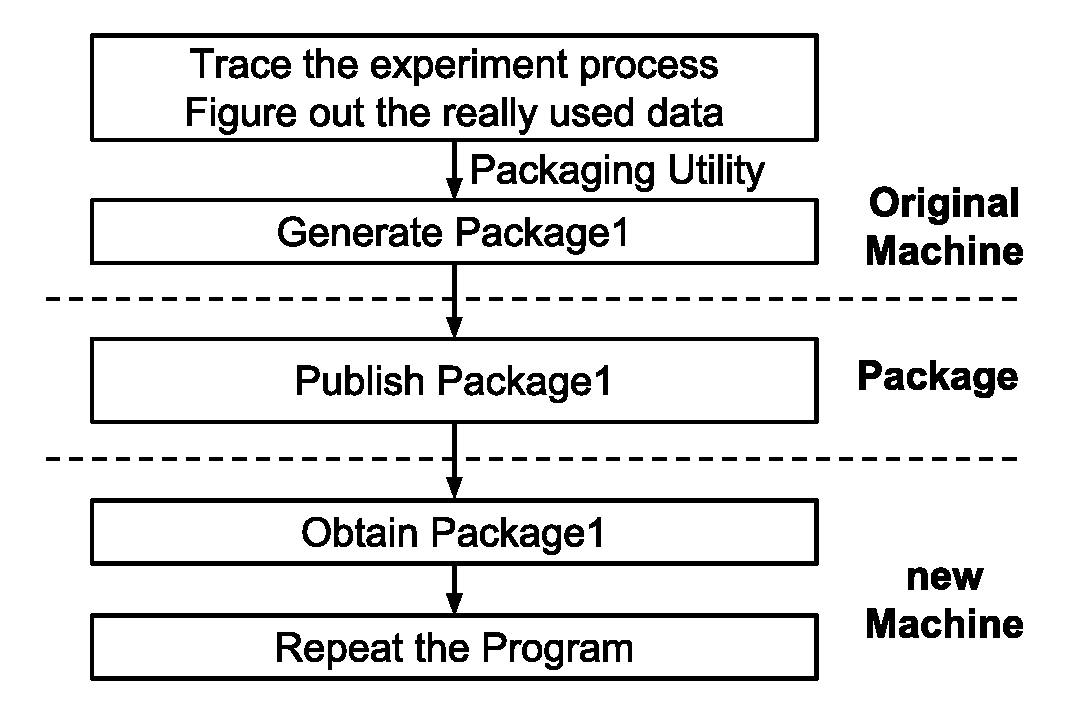
\includegraphics[width=.5\textwidth]{solution3.eps}
%\caption{Relationship of Roles}
%\label{fig:solution3}
%\end{figure}
%
%The relationship of different roles involved in the application preservation and
%reproduction is shown in Figure~\ref{fig:solution3}.  The original author uses the packaging utility to generate the package for one application.
%Then the package, together with
%its map file and description file will be published. When
%another researcher wants to repeat the application, one copy of the package will be downloaded into the new machine and the application can be repeated.
%
%When we try to repeat one application on one new machine, one map file is necessary for the relocation of the data access targets, as
%show in Figure~\ref{fig:version-evolution}. 
%The map file clearly defines the real location of each dependency in the format of dependency variables - the real location of dependency variable {\tt GIT} is \path{/data/git/cms-ttH} and the real location of dependency variable {\tt CVMFS}
%is {\tt /data/cvmfs/grid.cern.ch}.
%The script only refers to the dependency variables defined in the map file.
%This design decouples the application script and the actual data access targets, which minimizes the impact of the evolution of different data dependencies
%and ensures the transparent access.
%The modification of the package only introduces the minimal changes of the map file on the client side.
%
%This basic approach to dependency management is a step in the right direction
%for dependencies that are \emph{explicit} and \emph{external} to the
%user's native execution environment.  However, it leaves two other problems unsolved.
%
%First, the basic approach requires that someone be \emph{aware} of the dependencies,
%whether it be the end user, the system administrator, or the archive curator.
%It seems reasonable to expect the user to be aware of a large dependency mentioned in a top-level script.
%But, oftentimes the dependency is embedded invisibly deep within the software stack,
%or is connected to the machine by the local system administrators.  No single party
%is likely to have complete information about all of the dependencies.
%Second, the basic approach assumes that the entire dependency is actually
%consumed by the artifact.  As we have suggested above (and will show below),
%this sort of program often only consumes a small fraction of what it does declare
%as a dependency.
%
%To address both of these problems, users and curators alike need tools that
%will automatically observe the dependencies of complex applications, to
%facilitate automatic and efficient preservation.
%
